\documentclass{beamer}
\title{test of full size graphic}
\usepackage{tikz}
\usetheme{AnnArbor}

\begin{document}

\begin{frame}
    \maketitle
    Notice the fancy presentation theme.
\end{frame}

{ % all template changes are local to this group.
    \setbeamertemplate{navigation symbols}{}
    \begin{frame}[plain]
        \begin{tikzpicture}[remember picture,overlay]
            \node[at=(current page.center)] {
                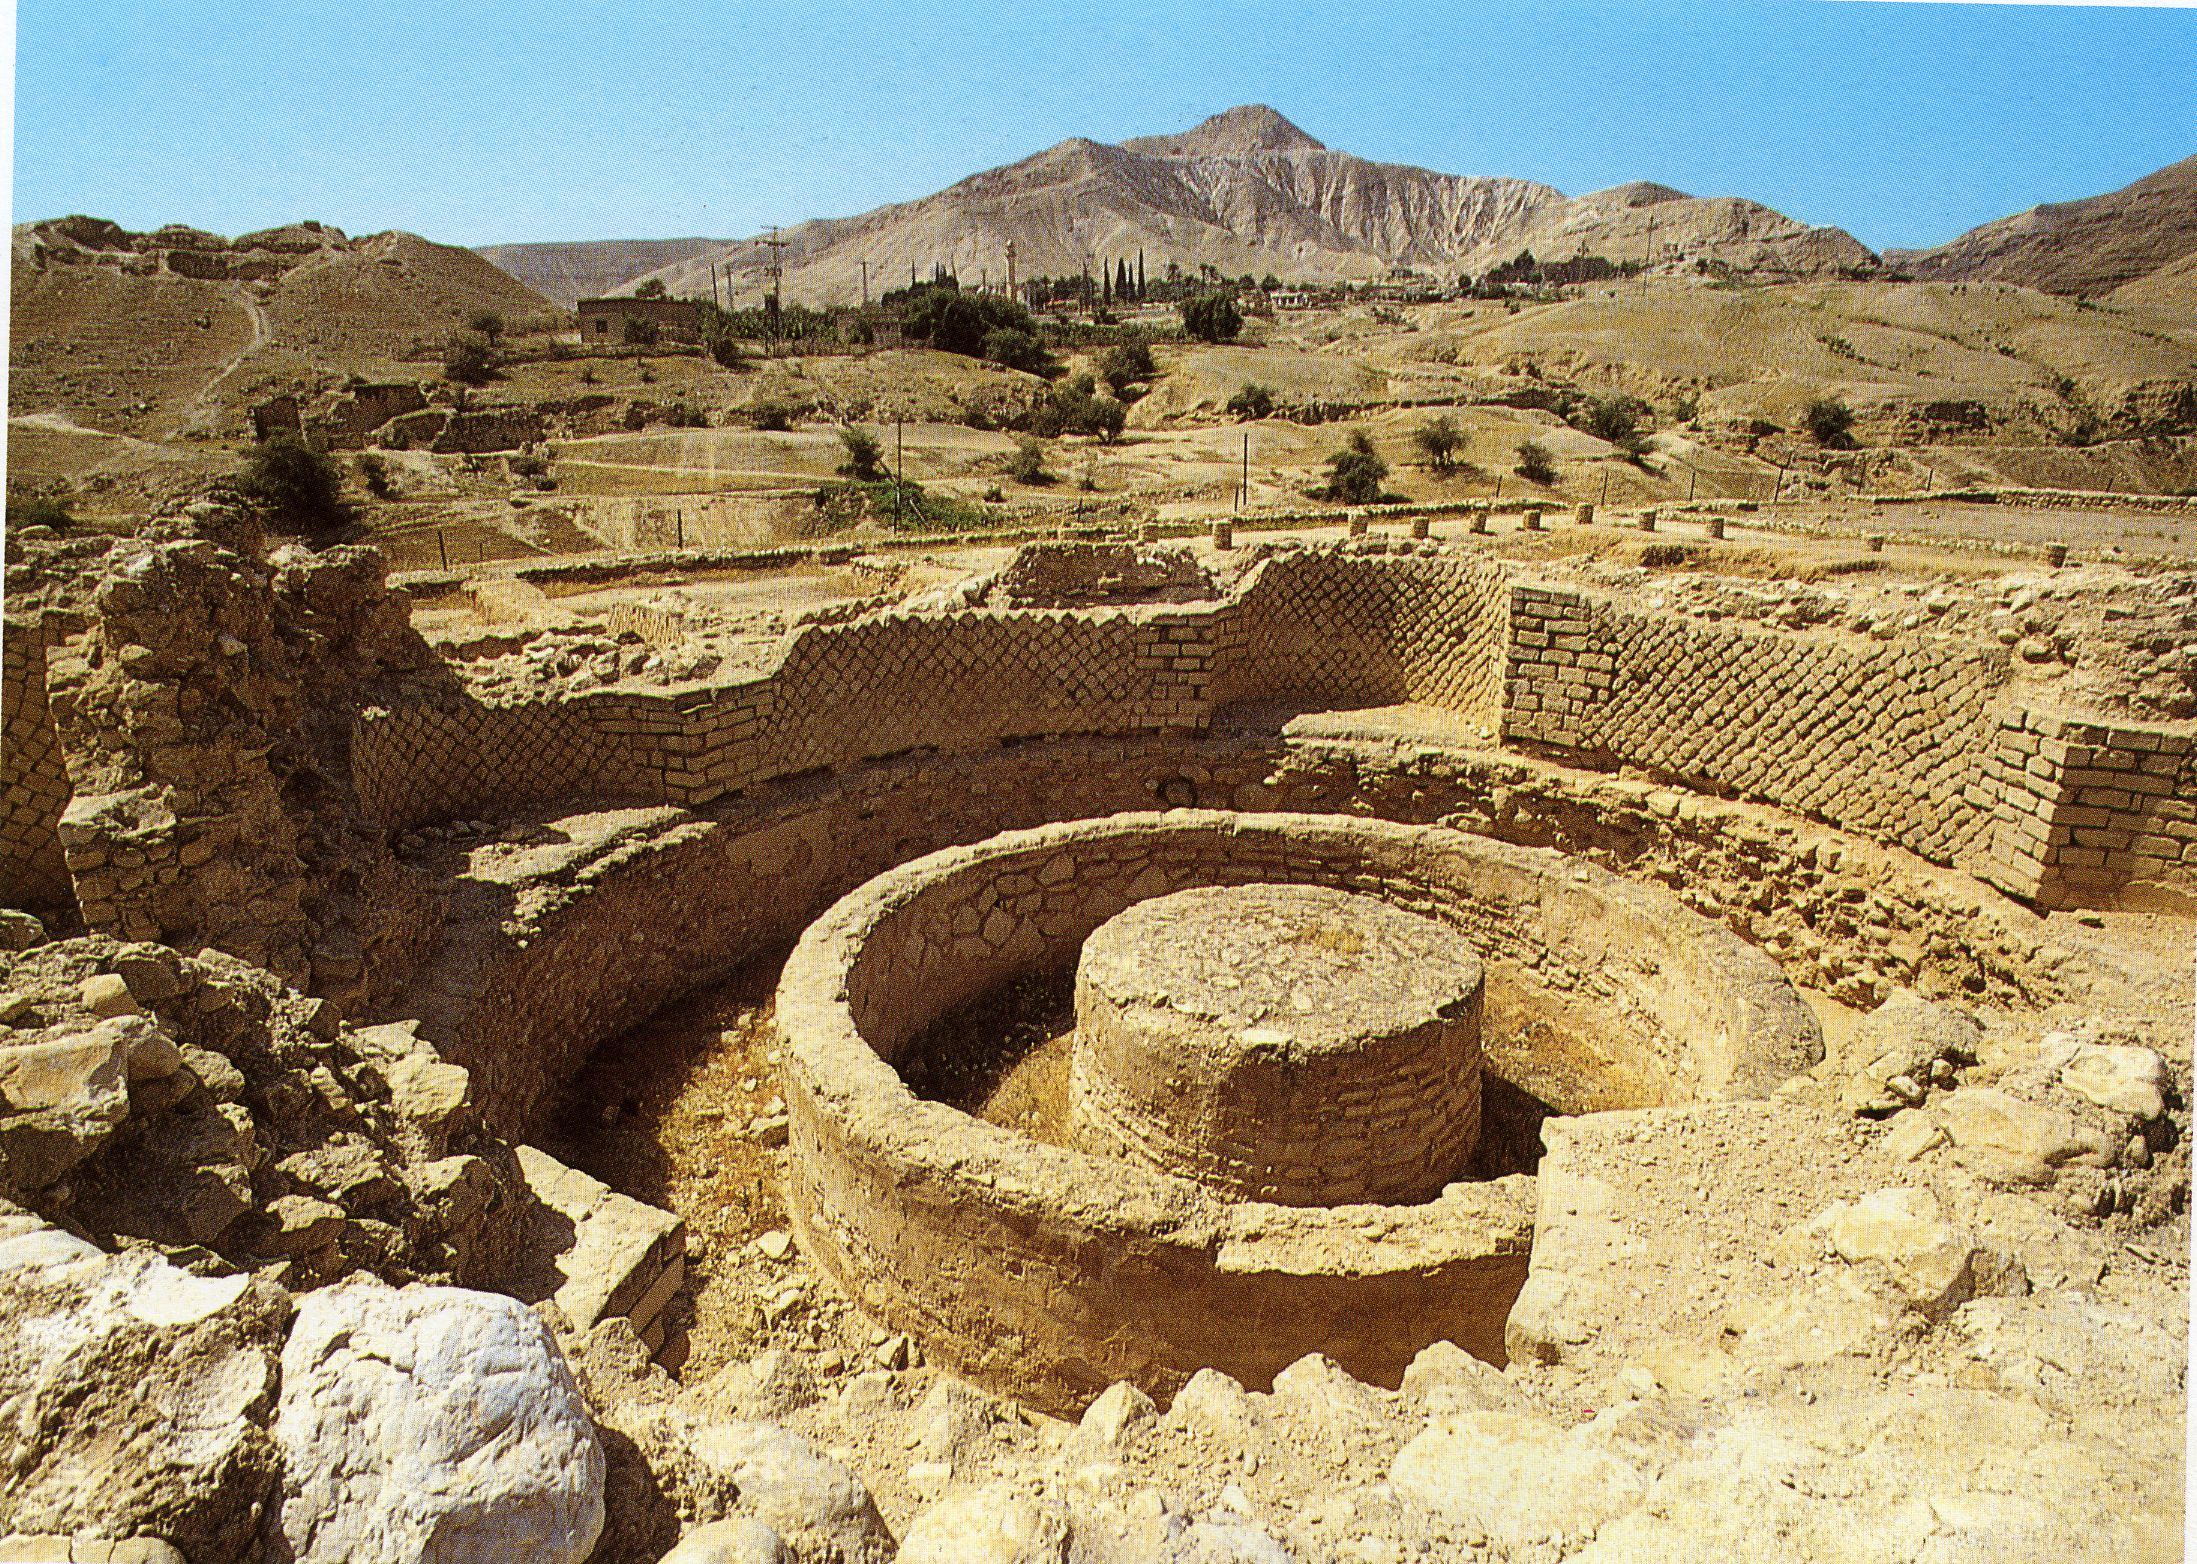
\includegraphics[width=\paperwidth]{jericho1.jpg}
            };
        \end{tikzpicture}
     \end{frame}
}

{ % all template changes are local to this group.
    \setbeamertemplate{navigation symbols}{}
    \begin{frame}[plain]
        \begin{tikzpicture}[remember picture,overlay]
            \node[at=(current page.center)] {
                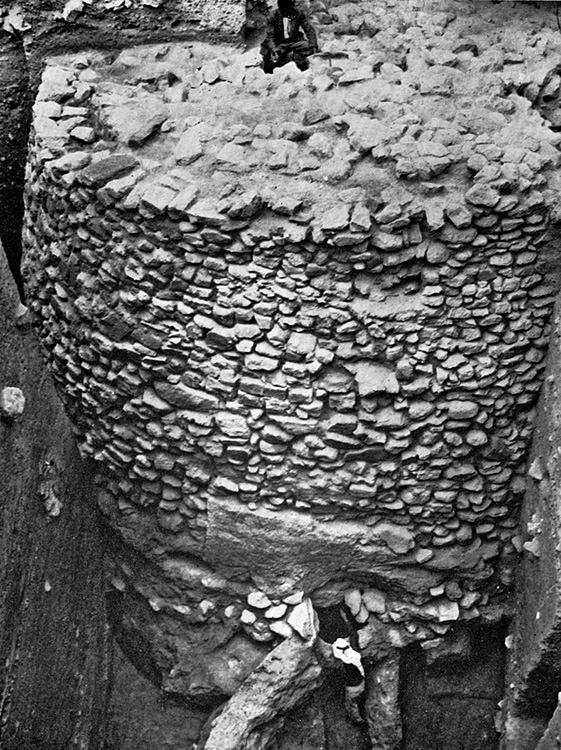
\includegraphics[height=\paperheight]{jerichoTower_1.jpg}
            };
        \end{tikzpicture}
     \end{frame}
}

\begin{frame}
    symbols should be back now
\end{frame}

\end{document}